\subsection{MBD and jet time distributions}
Figure~\ref{fig:jet_mbd_time} compares the leading jet time and MBD time distributions for events with uncalibrated leading jet $p_{T}$ between 20 and 60~GeV that do (red, blue) and do not (green) pass the energy fraction cut.
The MBD time is fairly consistent between the sample with the energy fraction jet background cut applied (red for only 1.5mrad runs and blue for all runs) and the sample without the energy fraction jet background cut applied (green).
The leading jet time is consistent between the two samples passing the energy fraction jet background cut.
However, the no background cut sample has a wider time distribution compared to the cleaner jet samples. 

\begin{figure}
    \centering
    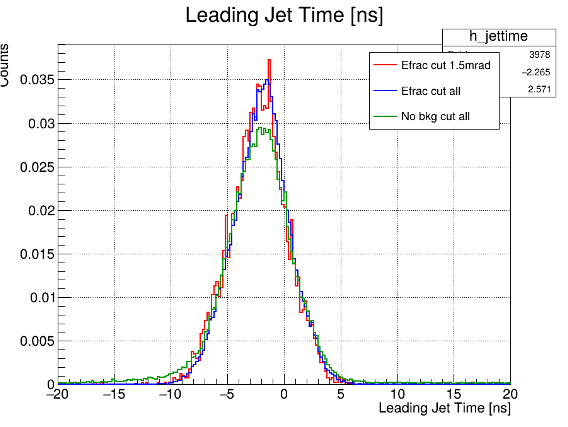
\includegraphics[width=0.48\linewidth]{Figures/jet_bkg_cuts/leading_jet_time.png}
    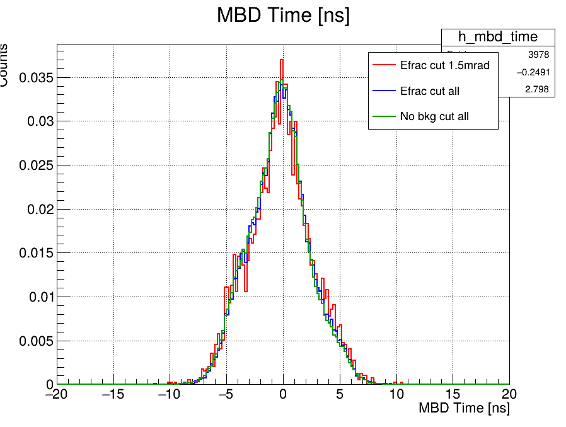
\includegraphics[width=0.48\linewidth]{Figures/jet_bkg_cuts/mbd_time.png}
    \caption{Leading jet time (left) and MBD time (right) distributions for events with uncalibrated leading jet $p_{T}$ between 20 and 60~GeV that do (red, blue) and do not (green)pass the energy fraction cut.}
    \label{fig:jet_mbd_time}
\end{figure}

The leading jet--MBD time difference for events passing and not passing the energy fraction cut is also studied and shown in Figure~\ref{fig:jet_mbd_time_diff}.
Once again, similar to the leading jet time distribution, the background events (events that do not pass the energy fraction cut) have a wider time distribution compared to the signal events (events that pass the energy fraction cut).
\begin{figure}
    \centering
    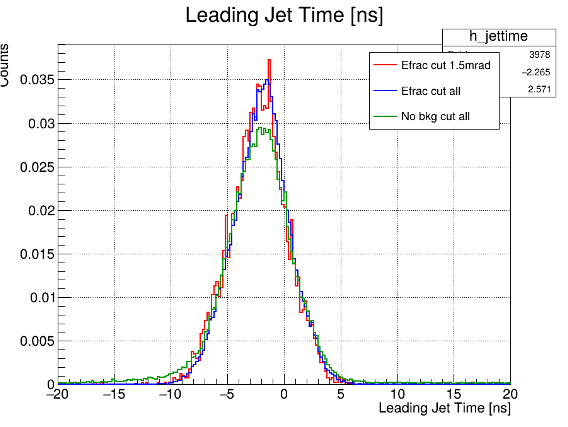
\includegraphics[width=0.48\linewidth]{Figures/jet_bkg_cuts/leading_jet_time.png}
    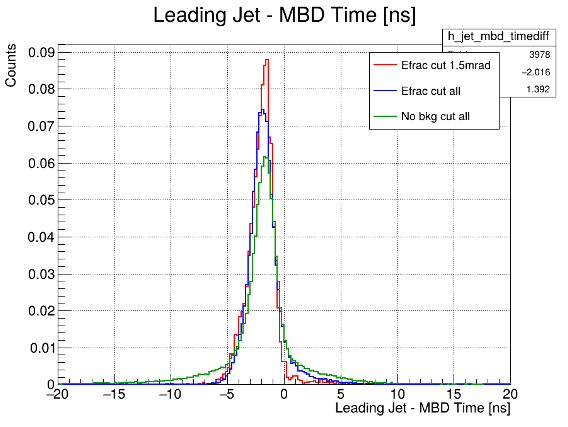
\includegraphics[width=0.48\linewidth]{Figures/jet_bkg_cuts/jet_mbd_timediff.png}
    \caption{Leading jet time (left) and leading jet--MBD time difference (right) distribution for events with uncalibrated leading jet $p_{T}$ between 20 and 60~GeV that do (red, blue) and do not (green) pass the energy fraction cut.}
    \label{fig:jet_mbd_time_diff}
\end{figure}

Figure~\ref{fig:jet_mbd_time_corr} shows the leading jet time and MBD time correlation for four sets of events: jet events in the 1.5 mrad dataset that pass the energy fraction cut, jet events in the full (0 mrad + 1.5 mrad) dataset that pass the energy fraction cut, jet events in the full dataset with no background cuts and jet events in the full dataset that do not pass the energy fraction cut.
Here a few trends emerge: first that for the events that pass the energy fraction cut, there is a clear correlation between the leading jet time and MBD time.
Second, that for events that do not pass the energy fraction cut, there is a large selection of events without a clear correlation between the leading jet and MBD time.
In the events that do not pass the energy fraction cut, there is also a clear correlation band. This in part can be attributed to the energy fraction cut cutting out good/real jet and especially photon jet events.
Finally, an excess on the right side of the correlation band is observed for the full dataset that is not observed in the 1.5 mrad dataset. 
This excess is due to the higher rate of pileup events in the full dataset compared to the 1.5 mrad dataset.
In pileup events, the MBD time is shifted to earlier times than the collisions due to the MBD timing algorithm using information on either side of the MBD detector. 
This excess also manifests in the leading jet--MBD time difference distribution for times greater than 0~ns.

\begin{figure}
    \centering
    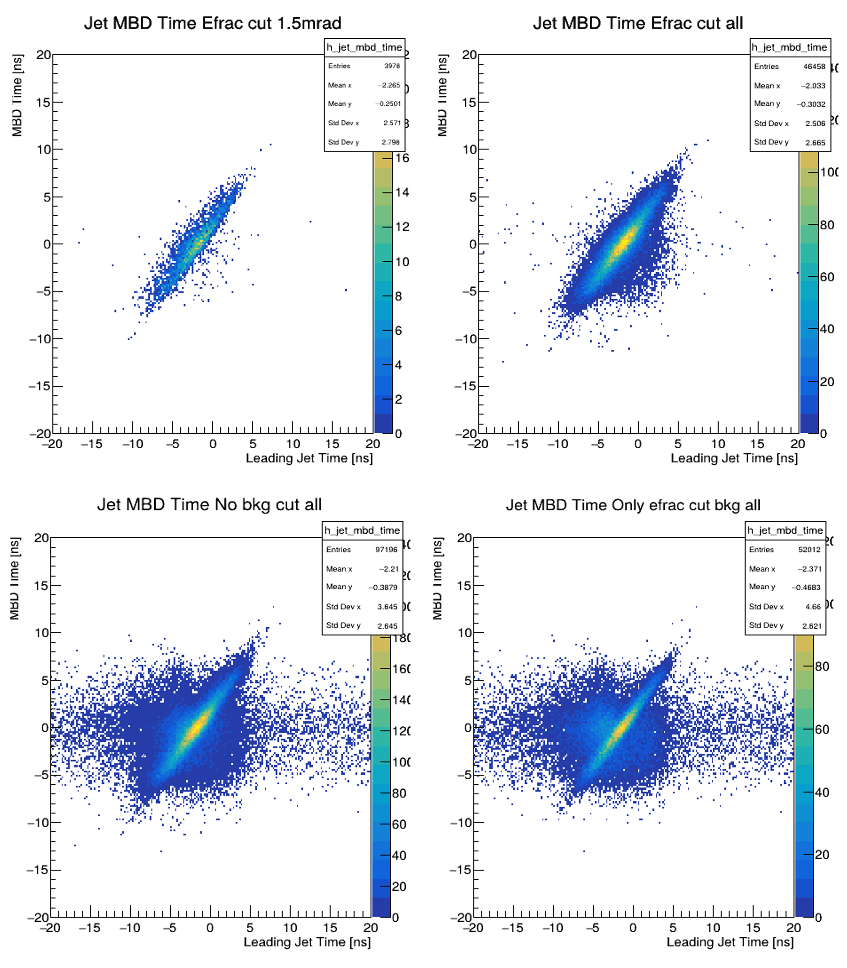
\includegraphics[width=\linewidth]{Figures/jet_bkg_cuts/jet_mbd_time_corr.png}
    \caption{Leading jet time and MBD time correlation for four sets of events: jet events in the 1.5 mrad dataset that pass the energy fraction cut (top left), jet events in the full (0 mrad + 1.5 mrad) dataset that pass the energy fraction cut (top right), jet events in the full dataset with no background cuts (bottom left) and jet events in the full dataset that do not pass the energy fraction cut (bottom right).}
    \label{fig:jet_mbd_time_corr}
\end{figure}

The $p_{T}$ dependence of the background contribution is also studied and shown in Figure~\ref{fig:jet_mbd_pt}. 
The major takeaway from studying the $p_{T}$ dependence is that the signal distribution remains stable across the jet $p_{T}$ ranges, but both the background to signal ratio and the background purity increases with increasing jet $p_{T}$. 
However, this level of background purity is not as important to the analysis since the energy fraction cut is applied and removes these background events in the actual analysis procedure.
It is good to see that the signal distribution is stable across the jet $p_{T}$ ranges and this reinforces that the simulation-based jet background cuts like the energy fraction cut are still needed in addition to the data-driven timing cuts.

\begin{figure}
    \centering
    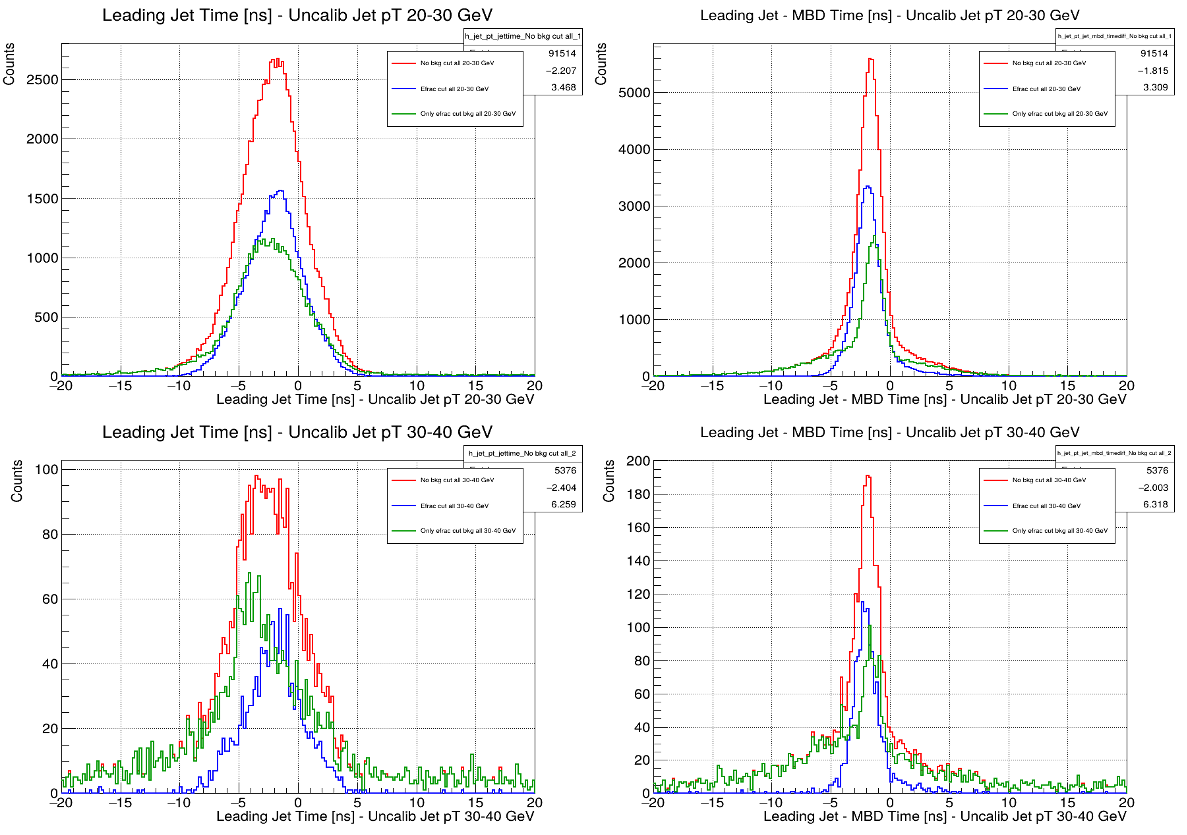
\includegraphics[width=\linewidth]{Figures/jet_bkg_cuts/time_cut_pt_dependence.png}
    \caption{Leading jet time (left) and Jet--MBD time difference (right) distributions for events with uncalibrated leading jet $p_{T}$ between 20 and 30~GeV (top) and 30 and 40~GeV (bottom) for events that do (blue) and do not (green) pass the energy fraction cut. The total distributions are also shown in red.}
    \label{fig:jet_mbd_pt}
\end{figure}